\documentclass[12pt,a4paper]{monografia}
\usepackage[english,brazilian]{babel}
\usepackage[utf8]{inputenc}
\usepackage[T1]{fontenc}
\usepackage{amsmath,amsthm,amsfonts,amssymb,textcomp}
%\usepackage{latexsym}
\usepackage{graphicx}
\graphicspath{{figuras}}
\usepackage{subfigure}
\usepackage{float}
\usepackage{longtable}
\usepackage{color}
\usepackage{epstopdf}
\usepackage{pdflscape}
\usepackage[breaklinks=true]{hyperref}
\usepackage[comma,authoryear]{natbib}
\usepackage[nonumberlist]{glossaries}
\usepackage{arydshln}
\usepackage{tablefootnote}
%\usepackage[alf]{abntcite}

%%% newcommand %%%%%%%%%%%%%%%%%
\newcommand{\PE}{Perkin-Elmer}
\newcommand{\BC}{Boller \& Chivens}

\newcommand{\degr}{\ensuremath{^{\circ}}}%                    % degree symbol:  °
\newcommand{\arcmin}{\ensuremath{^{\prime}}}%                    % degree symbol:  °
\newcommand{\fs}{\mbox{\ensuremath{.\!\!^s}}}
\newcommand{\farcm}{\mbox{\ensuremath{.\mkern-4mu^\prime}}}%    % fractional arcminute symbol: 0.'0
\newcommand{\farcs}{\mbox{\ensuremath{.\!\!^{\prime\prime}}}}%  % fractional arcsecond symbol: 0.''0
\newcommand{\fdg}{\mbox{\ensuremath{.\!\!^\circ}}}%             % fractional degree symbol:     0.°0




\makeglossaries



\newglossaryentry{Offset}{name={Offset}, description={Diferença entre a posição obtida pela redução da observação e a posição dada pela efeméride}}
\newglossaryentry{OPD}{name={OPD}, description={Observatório do Pico dos Dias - Brasópolis, MG}}
\newglossaryentry{LNA}{name={LNA}, description={Laboratório Nacional de Astrofísica - Itajubá, MG}}
\newglossaryentry{OHP}{name={OHP}, description={Observatoire Haute Provence - Saint-Michel-l'Observatoire, França}}
\newglossaryentry{RA}{name={RA}, description={Sigla para Ascensão Reta ($ \alpha $)}}
\newglossaryentry{DEC}{name={DEC}, description={Sigla para Declinação ($ \delta $)}}
\newglossaryentry{Anomalia Verdadeira}{name={Anomalia Verdadeira}, description={Ângulo formado entre o Periastro e a posição instantânea do objeto na órbita centrado no planeta e contada na direção do movimento orbital}}

\begin{document}
\doutorado

\titulo{Um Estudo Astrométrico e Fotométrico do Sistema Solar Exterior}
\autor{Altair Ramos Gomes Júnior}
\ultimonome{Gomes Júnior}
\nome{Altair Ramos}
\orientador{Marcelo Assafin}
\ttorientador{Professor Doutor}
\curso{Astronomia}
\instituicao{Universidade Federal do Rio de Janeiro}
\sigla{UFRJ}
\unidadeacademica{Centro de Ciências Matemáticas e da Natureza\\Observatório do Valongo}
\ano{2015}
\data{Junho de 2015}
\cidade{Rio de Janeiro}
\examinadorum{Primeira Pessoa}
\examinadordois{Segunda Pessoa}
\examinadortres{Terceira Pessoa}
\examinadorquatro{Quarta Pessoa}
\ttexaminadorum{Doutor}
\ttexaminadordois{Doutor}
\ttexaminadortres{bacharel}
\ttexaminadorquatro{licenciado}
\CDU{521.9}
\areas{Astrometria}
\npaginas{160}

\maketitle

%\begin{agradecimento}{Dedicatória}
%\indent \indent Agradeço à minha mãe Adelma e meu pai Altair por todo o apoio emocional e financeiro durante a minha trajetória acadêmica. Ao meu irmão, que sempre me incentivou, aos meus amigos e colegas pela troca de experiências.\\
%\indent À minha tia Maria do Carmo pelo auxílio dado para minha permanência no Rio de Janeiro, sem a qual não teria sido possível ficar no curso.\\
%\indent Ao meu orientador Marcelo Assafin por ter me aceito como aluno e me dado a oportunidade de trabalhar com as empolgantes áreas de Astrometria e Sistema Solar e por sua paciência ao me ensinar e me atualizar sobre o campo de trabalho.
%\end{agradecimento}

%\newpage
%\begin{epigrafe}
%"Queremos ter certezas e não dúvidas, resultados e não experiências, mas nem mesmo percebemos que as certezas só podem surgir através das dúvidas e os resultados somente através das experiências."\\
%\hfill Carl Gustav Jung
%\end{epigrafe}

\resumo{Resumo}
%\indent \indent O estudo da estrutura e evolução do Sistema Solar tem muita importância atualmente, por exemplo, na compreensão dos mecanismos de formação dos planetas de outras estrelas (exoplanetas), trazendo em seus desdobramentos valiosas informações quanto a viabilidade de formação de ambientes que comportem vida.

%Praticamente cada satélite é um problema particular de Mecânica Celeste. Dessa forma, a observação de seus movimentos é muito útil por razões teóricas. A preparação e realização de missões espaciais para alguns planetas, e mesmo alguns satélites, como Titã de Saturno ou os Galileanos de Júpiter, requer observações frequentes e posições muito acuradas de todos os satélites do sistema planetário visitado.\\
%\indent Os satélites irregulares de planetas gigantes, principalmente de Júpiter e de Saturno, são substancialmente menores do que os satélites regulares e possuem órbitas mais distantes, excêntricas, inclinadas e, na maioria dos casos, retrógradas. Explicar a existência dos satélites irregulares dos planetas gigantes é um estudo interessante em dinâmica orbital.\\
%\indent É amplamente aceito que eles, devido à configuração orbital, foram capturados por seus planetas. Porém, ainda não são certos a origem e o método de captura desses objetos embora as teorias mais prováveis sejam a de arrasto gasoso durante a formação do Sistema Solar e a captura de três corpos.\\
%\indent A maioria dos satélites formam famílias com características orbitais semelhantes sugerindo uma evolução dada por colisões. A compreensão desses mecanismos nos fará entender melhor o nosso próprio sistema solar e, possivelmente, de sistemas extra-solares.\\
%\indent Com o pacote astrométrico PRAIA o tempo empregado na redução de grandes quantidades de imagens foi diminuído significativamente. Os objetivos científicos dos nossos programas observacionais agora tem sido atingidos em curtíssimo prazo, em consonância com a atual demanda astronômica e astrofísica de nossa área.\\
%\indent Em uma base de dados com mais de 100 mil imagens obtidas entre 1992 e 2012 no telescópios de 1.2m do Observatoire de Haute Province, França, e nos telescópios \PE, \BC{} e Zeiss no Observatório do Pico dos Dias, mais de 4 mil contem satélites irregulares de Júpiter e Saturno. Reduzir essa grande quantidade de observações com precisão só foi possível com a utilização do PRAIA. Como é possível ver nos resultados obtidos, os offsets de posição refletem o erro natural da astrometria e o erro das efemérides dos satélites mais fracos, e sugerem que podemos efetivamente contribuir para que novas integrações numéricas forneçam posições mais precisas. Essas novas efemérides irão permitir que ocultações estelares por esses objetos possam ser preditas com maior precisão. A observações dessas ocultações permitirão um maior conhecimento das propriedades físicas dos satélites. 

\par
\vspace{1em}
\noindent\textbf{Palavras-chave:} Astrometria, Ocultações


\tableofcontents % para gerar o sumário
\thispagestyle{empty} % para que a pagina não seja enumerada
%\listoffigures % cria a lista de figuras
%\thispagestyle{empty}
%\listoftables % cria a lista de tabela
%\thispagestyle{empty}

\pagestyle{ruledheader}

\chapter{Introdução}
\label{Cap: intro}

\indent \indent O estudo de objetos como TNOs, Centauros e Satélites Irregulares (remanescentes relativamente inalterados da formação do sistema solar) nos ajudam a compreender a formação e evolução do Sistema Solar. Atualmente, é aceito que TNOs e Centauros tenham sido formados nas partes mais internas do sistema solar. Eles teriam então sido colocados em suas posições atuais devido a troca de momento angular entre os planetas e planetésimos quando da migração dos planetas gigantes. A evolução se deu de tal forma que a passagem dos planetesimais e planetas por zonas de ressonância de movimento médio redefiniu as órbitas desses corpos \citep{Tsiganis2005}.\\
\indent Sabe-se que poucas sondas espaciais foram enviados para estudar o Sistema Solar Externo e que a quantidade de objetos estudados é muito pequena. Por isso, ainda hoje, as observações de solo tem se mostrado de grande importância.\\
\indent Os sistemas de Júpiter e Saturno já foram pelas Voyager I e II, Galileu (Júpiter) e Cassini (Saturno), porém apenas Saturno continua sendo investigado por uma sonda. Porém as sondas observaram apenas os planetas, os anéis e satélites mais internos. Os satélites externos, que acredita-se ser oriundo de capturas ou foram pouco observados (como Phoebe) ou simplesmente não foram observados.\\
\indent Já no caso de Urano e Netuno, nenhuma sonda exclusiva foi enviada, apenas as Voyagers I e II os visitaram, mas não permaneceram nos sistemas. A sonda New Horizons já está próxima a Plutão e obterá parâmetros físicos para Plutão e seus satélites (primeira visita por sonda a um objeto do cinturão de Kuiper), porém será uma passagem rápida e o acompanhamento da evolução do sistema, incluindo a evolução da atmosfera de Plutão se dará por observações de solo.\\
\indent A quantidade de objetos descobertos além da órbita de Saturno tem aumentado muito desde o fim do século passado. Como são raras as oportunidades em que uma sonda se aproxima desses objetos, a obtenção de suas características físicas ficam a cargo de observações de solo ou de
telescópios espaciais.\\
\indent Um método que tem se mostrado eficiente para a obtenção desses parâmetros é o métodode ocultações estelares, que proporciona medidas tão precisas que são apenas superadas por medidas oriundas de sondas.

\chapter{Astrometria dos satélites irregulares dos planetas gigantes}
\label{Cap: Irr-astrometria}

\indent \indent Os satélites irregulares dos planetas gigantes são menores que as regulares, possuindo órbitas mais excêntricas, inclinadas e distantes. Na maioria dos casos, essas órbitas são retrógradas. Devido suas configurações orbitais, é altamente aceito que estes objetos foram capturados nos estágios iniciais da formação do sistema solar \citep{Sheppard2003}.

Por serem pequenos, eles são pouco brilhantes e só foram descobertos no último século\footnote{Website: http://ssd.jpl.nasa.gov/?sat\_discovery}. Dentre os satélite irregulares dos planetas gigantes, poucos são aqueles que possuem medidas de seus parâmetros físicos. Apenas Himalia, Phoebe e Nereida foram observados por sondas, apesar de não serem medidas ideais, já que foram alvos de oportunidade. A sonda Cassini observou Himalia em 2000 ao passar próximo a Júpiter e obteve o tamanho de Himalia com um erro médio de 10 km \citep{Porco2003}. Em 2004, a Cassini, aproximando-se de Saturno, observou Phoebe em alta resolução obtendo um erro médio na medida de seu tamanho de 0.7 km \citep{Thomas2010}. Por fim, Nereida foi observado em 1989 pela sonda Voyager 2 e seu tamanho foi obtido com um erro de 25 km \citep{Smith1989}. Para outros satélites irregulares de Júpiter, seus tamanhos foram estimados por \cite{Rettig2001} impondo um albedo de 4\% cam a justifica de que esse valor é um albedo nominalmente utilizado para objetos do Sistema Solar Externo.

Existem alguns mecanismos de captura de objetos por planetas gigantes propostos na literatura. Há o Arrasto Gasoso na nebulosa circumplanetária primordial \citep{Sheppard2005} onde o movimento objeto seria afetado gás e sua velocidade diminuiria até que fosse capturado pelo planeta. Outro mecanismo se chama captura pull-down \citep{Sheppard2005}, onde a massa do planeta aumentaria enquanto o objeto estivesse temporariamente capturado.

Um mecanismo baseado no modelo de Nice \citep{Morbidelli2005, Tsiganis2005, Gomes2005} foi proposto por \cite{Nesvorny2007} e, especificamente para Júpiter, por \citealp{Nesvorny2014}. Durante a instabilidade do sistema solar primordial, ocorreram encontros entre os planetas externos. Esses encontros planetários poderiam trocar energia e momento angular entre os planetas e os objetos próximos tornando possível a captura de um corpo irregular por um planeta gigante. Nesse cenário, a taxa de sobrevivência de satélites anteriores ao LHB (Bombardeamento Pesado Tardio\footnote{"Late Heavy Bombardment", em inglês}) é muito pequena.

Um outro mecanismo importante é a captura através de interações colisionais \citep{Sheppard2005}. Uma colisão entre dois corpos pequenos dentro da esfera de Hill do planeta poderia gerar objetos fragmentados e a energia dissipativa poderia ser tal que alguns desses objetos seriam capturados.

Alguns desses objetos formam grupos dinâmicos com elementos orbitais semelhantes, chamados famílias, similar às famílias encontradas no Cinturão Principal de Asteróides. Essas famífias podem ter sido criadas por um corpo pai que se fragmentou por colisões com cometas ou outros asteróides \citep{Nesvorny2004}. Colisões com cometas tem uma probabilidade maior de ocorrer durante o Bombardeamento Pesado Tardio (LHB) \citep{Gomes2005}.

\cite{Nesvorny2003} estudou as taxas de colisões entre satélites irregulares e concluiu que alguns satélites podem ter sido removidos por colisão com um satélite maior. A taxa de colisão entre os satélites do grupo de Himalia (Himalia, Elara, Lysithea and Leda, principalmente), por exemplo, foi encontrado como sendo maior que "um" durante a idade do sistema solar sugerindo que sua estrutura atual foi originada por colisão satélite-satélite.

Para Phoebe, materiais ejetados de sua superfície causadas por impactos poderiam evoluir devido ao arrasto de Poynting-Robertson e colidir com Iapetus causando causando a grande variação de albedo observada no satélite \citep{Nesvorny2003}. De fato, A Cassini detectou em Phoebe uma característica de absorção em 2.42 $\mu m$, provavelmente combinações de CN, que foi também detectada no lado escuro de Iapetus \citep{Clark2005}

Se esses objetos foram capturados, permanece a pergunta de onde eles vieram. \citealp{Clark2005} mostraram a partir de espectroscopia da Cassini que Phoebe tem uma superfície provavelmente coberta por materiam do sistema solar externo e \citealp{Grav2003} mostraram que os satélites de grupo prógrado de Júpiter Himalia tem cores cinzas implicando que suas superfícies são similares a asteróides tipo C. Nesse mesmo trabalho, o grupo retrógrado de Júpiter Carme foi encontrado como tendo cores superficiais semelhantes à asteróides tipo D como a família de Hilda ou famílias de troianos, enquanto JXIII Kalyke tem uma cor mais avermelhada como centauros ou objetos trans-Netunianos (TNOs).

Para os satélites de saturno, \citealp{Grav2007} mostraram através de suas cores e inclinações espectrais que esses satélites contêm uma fração mais ou menos igual de objetos semelhantes a asteróides tipo c, P e D, mas SXXII Ijiraq é um pouco mais avermelhado que objetos tipo D. Esses trabalhos sugerem origins diferentes para os satélites irregulares.

Nesse contexto, durante o mestrado, foi realizado junto ao grupo um trabalho de caráter astrométrico para a melhoria das efemérides dos satélites irregulares de Júpiter Saturno. Em colaboração com o Dr. Jean-Eudes Arlot do IMCCE, reduzi um banco de dados observado no Observatoire Haute-Provence (OHP) entre 1998 e 2008, contendo mais de 28 mil posições para 10 satélites. Reduzi também um banco de dados com mais de 100 mil imagens obtidas no Observatório do Pido dos Dias (OPD) entre 1992 e 2014. Já no doutorado, neste mesmo âmbito, reduzi 810 observações feitas no European Southern Observatory (ESO) em 24 noites utilizando o detector mosaico CCD Wide Field Imager (WFI).

Mais de 8000 posições foram identificadas como pertencentes a satélites irregulares. Porém, devido à grande gama de configurações (3 sítios, 5 telescópios, mais de 10 câmeras e mais de 10 filtros) e às condições observacionais de algumas noites, 6523 posições foram selecionadas como boas posições, ou seja, possuem 3 ou mais estrelas do catálogo de referência (UCAC4), estão dentro de 2$\sigma$ da dispersão das posições da noite e a dispersão da noite à qual pertence não é maior que 2$\sigma$ da média das dispersões das noites. Essa estatística é feita satélite por satélite. O trabalho está aceito para publicação \citep{GomesJunior2015-Irregular} e o catálogo de posições está disponível no CDS.

Um dos principais resultados desse trabalho foi a grande quantidade de posições obtidas para os satélites irregulares em comparação com a quantidade utilizada nas integrações numéricas atuais (ver tabela \ref{Tab: comparison-horizons}).

\begin{table}[h]
\caption{\label{Tab: comparison-horizons} Comparação entre o número de posições obtidas em \cite{GomesJunior2015-Irregular} e o número utilizado nas integrações numéricas das órbitas pelo JPL como publicado por  \cite{Jacobson2012}. Os satélites estão separados por planeta (linha reta) e por família orbital (linha tracejada)}
\begin{centering}
\begin{tabular}{lccccccc}
\hline  \hline
Satélite & Diâm. (km)\tablefootnote{Planetary Satellite Physical Parameters - JPL: \url{http://ssd.jpl.nasa.gov/?sat_phys_par}} & Mag V  & OPD  & OHP & ESO & Total  & Jacobson \tabularnewline
\hline
Himalia & 170 & 14 & 854 & 357 & 23 & 1234 & 1757 \tabularnewline
Elara & 86 & 16 & 403 & 187 & 46 & 636 & 1115 \tabularnewline
Lysithea & 36 & 18 & 60 & 84 & 90 & 234 & 431 \tabularnewline
Leda & 20 & 19 & 6 & 48 & 44 & 98 & 178 \tabularnewline
\hdashline
Pasiphae & 60 & 17 & 295 & 248 & 66 & 609 & 1629 \tabularnewline
Callirrhoe & 9 & 21 & 9 & -  &  16 & 25 & 95 \tabularnewline
Megaclite & 5 & 22 & - & -  &  10 & 10 & 50  \tabularnewline
\hdashline
Ananke & 28 & 18 & 52 & 141 & 57 & 250 & 600 \tabularnewline
Praxidike & 7 & 21 & - & -  &   2 & 2 & 59 \tabularnewline
\hdashline
Carme & 46 & 18 & 90 & 204 & 37 & 331 & 973 \tabularnewline
Sinope & 38 & 18 & 41 & 169 & 11 & 221 & 854 \tabularnewline
Themisto & 8 & 21 & - & - & 16 & 16 & 55 \tabularnewline
\hline
Phoebe & 213 & 16 & 1239 & 516 & 32 & 1787 & 3479 \tabularnewline
\hdashline
Siarnaq & 40 & 20 & - & 20 & 56 & 76 & 239 \tabularnewline
Paaliaq & 22 & 21 & - & - & 11 & 11 & 82 \tabularnewline
\hdashline
Albiorix & 32 & 20 & - & - & 46 & 46 & 137 \tabularnewline
\hline
Sycorax & 150 & 21 & - & - & 35 & 35 & 237 \tabularnewline
\hline
Nereid & 340 & 19 & 803 & - & 99 & 902 & 716 \tabularnewline
\hline
\end{tabular}
\par\end{centering}
\end{table}

Com o objetivo ver o potencial das nossas posições em melhorar as órbitas dos satélites irregulares, analizamos os offsets das nossas posições com respeito às efemérides do JPL. Tomando Carme como exemplo, plotamos os offsets médios das efemérides para cada noite na Fig. \ref{Fig: carme_anom} e suas respectivas dispersões (erro de barra 1$\sigma$) em função da anomalia verdadeira em ascenção reta e declinação. A figura mostra claramente um erro sistemático em declinação. Quando Carme está próximo a seu apojove (anomalia verdadeira = 180$\degr$), seus offsets tem maior probabilidade de serem mais negativos do que aqueles próximos ao seu perijove (anomalia verdadeira = 0$\degr$). Todos os offsets obtidos de observações feitas em quatro telescópios diferentes usando câmeras e filtros diferentes estão em bom acordo, o que significa que há um erro nas efemérides de Carme, muito provavelmente devido a um erro em sua inclinação orbital.

\begin{figure}[h]
\begin{centering}
\subfigure[Right Ascension]{\includegraphics[scale=0.45]{figuras/Carme_RA}\label{Fig: carme_alfa}}
\subfigure[Declination]{\includegraphics[scale=0.45]{figuras/Carme_DEC}\label{Fig: carme_delta}}
\caption{Offsets médios das efemérides e dispersões (barra de erro 1$\sigma$) nas coordenadas de Carme tomadas noite a noite por anomalia verdadeira para cada telescópio. O quadrado vermelho são as observações com o telescópio do OPD Perkin-Elmer, o círculo azul para o Boller \& Chivens também do OPD, o triângulo pra cima preto para o OHP e a estrela verde para o ESO.}
\label{Fig: carme_anom}
\end{centering}
\end{figure}

Esse padrão em declinação também foi identificado para outros satélites como Pasiphae e Ananke. Para alguns satélites a cobertura orbital não foi suficiente para indicar claramente a presença de erros sistemáticos em elementos orbitais específicos. Os gráficos para todos os satélites estão disponíveis em \cite{GomesJunior2015-Irregular}.

Um método que tem se mostrado eficiente para a obtenção desses parâmetros é o métodode ocultações estelares, que proporciona medidas tão precisas que são apenas superadas por medidas oriundas de sondas. Uma vez que suas efemérides não são muito precisas, predizer e observar ocultações estelares é muito difícil e nenhuma observação de um evento desses para um satélite irregular é encontrado na literatura. Um projeto nesse sentido está sendo encaminhado e será discutido na seção \ref{Sec: Irregulares}.


\chapter{Astrometria de Netuno e Tritão}
\label{Cap: Netuno}


\chapter{Ocultações Estelares}
\label{Cap: observacoes}

\indent \indent Ocultação estelar é um evento que ocorre quando um objeto do sistema solar passa na frente de uma estrela de forma que o brilho da estrela é completamente ou parcialmente apagado durante um intervalo de tempo. A variação de brilho da estrela pode ser medido fazendo-se observações com exposições curtas. O produto gerado é uma curva de luz luminosidade x tempo. Essa técnica pode ser utilizada para se obter parâmetros físicos dos objetos ocultantes como tamanho, densidade, detecção da presença de atmosfera, satélites ou anéis, etc \citep{Elliot1979}.

A Fig. \ref{Fig: occ-scheme}.1 mostra uma curva de luz esquemática de uma ocultação estelar central por um planeta com atmosfera e anéis. Ao ocultar a estrela, os anéis passarão primeiro, a densidade do anel, tamanho e tempo de exposição determinará a queda de brilho da estrela. Ao chegar no corpo principal, caso não possua atmosfera, a queda de brilho será abrupta, caso possua, a queda de brilho será mais suave devido à refração da luz da estrela na atmosfera dificultando a determinação da superfície do objeto.

\begin{figure}[h]
\begin{centering}
\includegraphics[scale=0.75]{figuras/stellarocc.png} 
\label{Fig: occ-scheme}
\caption{Curva de luz esquemática de uma ocultação estelar por um planeta com atmosfera e anéis. Fonte: \cite{Elliot1979}}
\end{centering} 
\end{figure}

A suavidade da curva portanto será determinada pelo gradiente de temperatura, pressão e densidade da atmosfera, presença de nuvens, etc. A luz da estrela nunca será completamente apagada quando ocultada por um objeto com atmosfera devido à refração da luz na atmosfera onde parte dela convergirá na direção do observador. Caso a ocultação seja central para o observador haverá um aumento de brilho no meio do evento pois a convergência da luz será máxima. A atmosfera, no caso, agiria como uma lente como mostrado na Fig. \ref{Fig: occ-scheme}.1.

Quando o evento é observado por diversos telescópios espalhados, cada observador verá a ocultação em latitudes diferentes. Essas diversas curvas de luz permitirá reconstruir a forma do objeto possivelmente identificando estruturas superficiais como montanhas e crateras. Como a estrela está muito distante, podendo ser considerada quase pontual, a sombra do objeto durante a ocultação é muito próximo ao seu tamanho real.

Para se observar esses eventos, portanto, é necessário uma campanha grande com observadores espalhados por várias regiões para cobrir a sombra do objeto. A precisão nas posições da estrela e do objeto são cruciais pois o evento ocorre em instantes específicos e passará por regiões específicas da Terra alheias à escolha do observador.

%Since their ephemerides are not very precise, predicting and observing stellar occultations are very difficult, and no observation of such an event for an irregular satellite is found in the literature. The precise star positions to be derived by the ESA astrometry satellite Gaia \citep{deBruijne2012} will render better predictions with the only source of error being the ephemeris. The positions derived from our observations can be used in new orbital numerical integrations, generating more precise ephemerides.

%The power of stellar occultations for observing relatively small diameter solar system objects is supported by recent works, such as the discovery of a ring system around the Centaur (10199) Chariklo \citep{Braga-Ribas2014}. Once irregular satellites start to be observed by this technique, it will be possible to obtain their physical parameters (shape, size, albedo, density) with unprecedented precision. For instance, in this case, sizes could be obtained with kilometer accuracy. The knowledge of these parameters would in turn bring valuable information for studying the capture mechanisms and origin of the irregular satellites.

\section{Ceres}
\label{Sec: Ceres}

\indent \indent Apesar de Ceres não ser um objeto do sistema solar exterior, ele é o único planeta-anão no sistema solar interno e, por isso, é um objeto de grande importância e seu estudo pode ter grande impacto na formação e evolução do sistema solar. Na verdade, foi proposto que a origem de Ceres pode ser como um objeto transnetuniano \citep{McKinnon2012}, espalhado posteriormente para o cinturão principal de asteroides devido à migração dos planetas gigantes predito pelo Modelo de Nice \citep{Gomes2005}. Mesmo que ele tenha sido formado próximo à sua localização atual, a história dinâmica do sistema solar deve ter deixado sua assinatura em Ceres.

Contendo aproximadamente um quinto de toda a massa do cinturão de asteroides, espera-se que Ceres esteja em equilíbrio gravitacional e seja, portanto, um elipsóide Maclaurin ou Jacobi. De fato, observações diretas de Ceres com a utilização de ótica adaptativa indica que ele é um esferóide achatado nos pólos \citep{Drummond2014}. O conhecimento preciso de seu tamanho e forma é extrema importância para modelos de densidade, estrutura interna e diferenciação.

A primeira ocultação estelar por Ceres foi observada em 1984 \citep{Millis1987} e determinou seu tamanho com precisão de alguns quilômetros em uma época que as incertezas eram, normalmente, dez vezes maiores. Devido ao brilho aparente de Ceres ser alto, comparado à maioria dos asteroides, estrelas capazes de causar uma queda de magnitude detectável quando ocultadas são limitadas às mais brilhantes. Por exemplo, depois do evento de 1984, apenas 4 ocultações estelares por Ceres foram observadas \citep{Dunham2014}. Duas delas tiveram apenas duas cordas cada que não foram suficientes para prover resultados acurados\footnote{Esses eventos ocorreram em 22 de Agosto de 1994 e 30 de Outubro de 2010.}. Os dois restantes, que ocorreram em 17 de Agosto de 2010 e 25 de Outubro de 2013, foram trabalhos por mim em colaboração com o grupo do Rio \citep[aceito]{GomesJunior2015-Ceres}.

Os dois eventos foram preditos por Steve Preston\footnote{Predições publicadas em \url{http://asteroidoccultation.com}.} para a IOTA (International Occultation Timing Association), durante predições de rotina de ocultações de asteroides de estrelas brilhantes. Os caminhos das sombras podem ser visualizados na Fig. \ref{Fig: Ceres-map}.

\begin{figure}[h]
\begin{centering}
\subfigure[Ocultação de 2010]{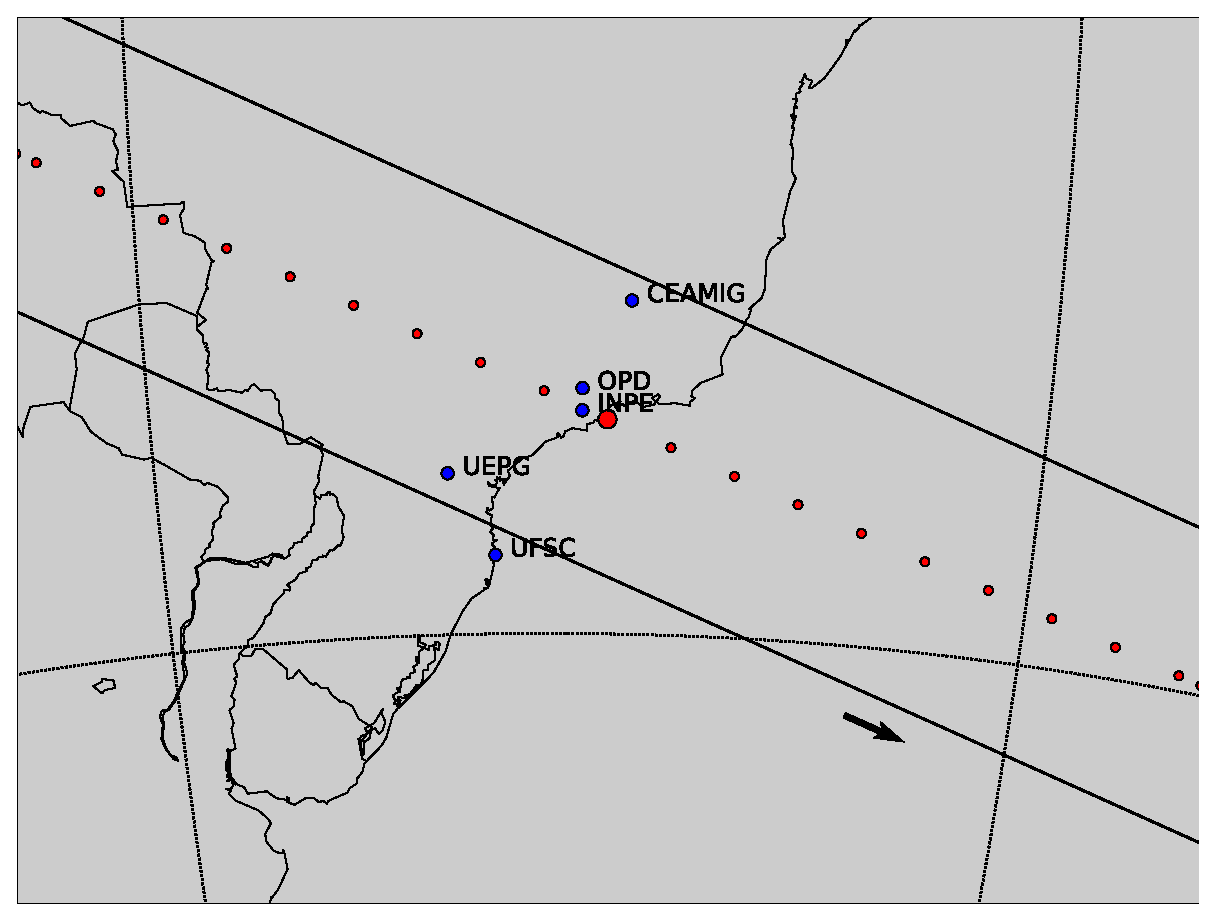
\includegraphics[scale=0.39]{figuras/Ceres_2010.eps}\label{Fig: Ceres-map-2010}}
\subfigure[Ocultação de 2013]{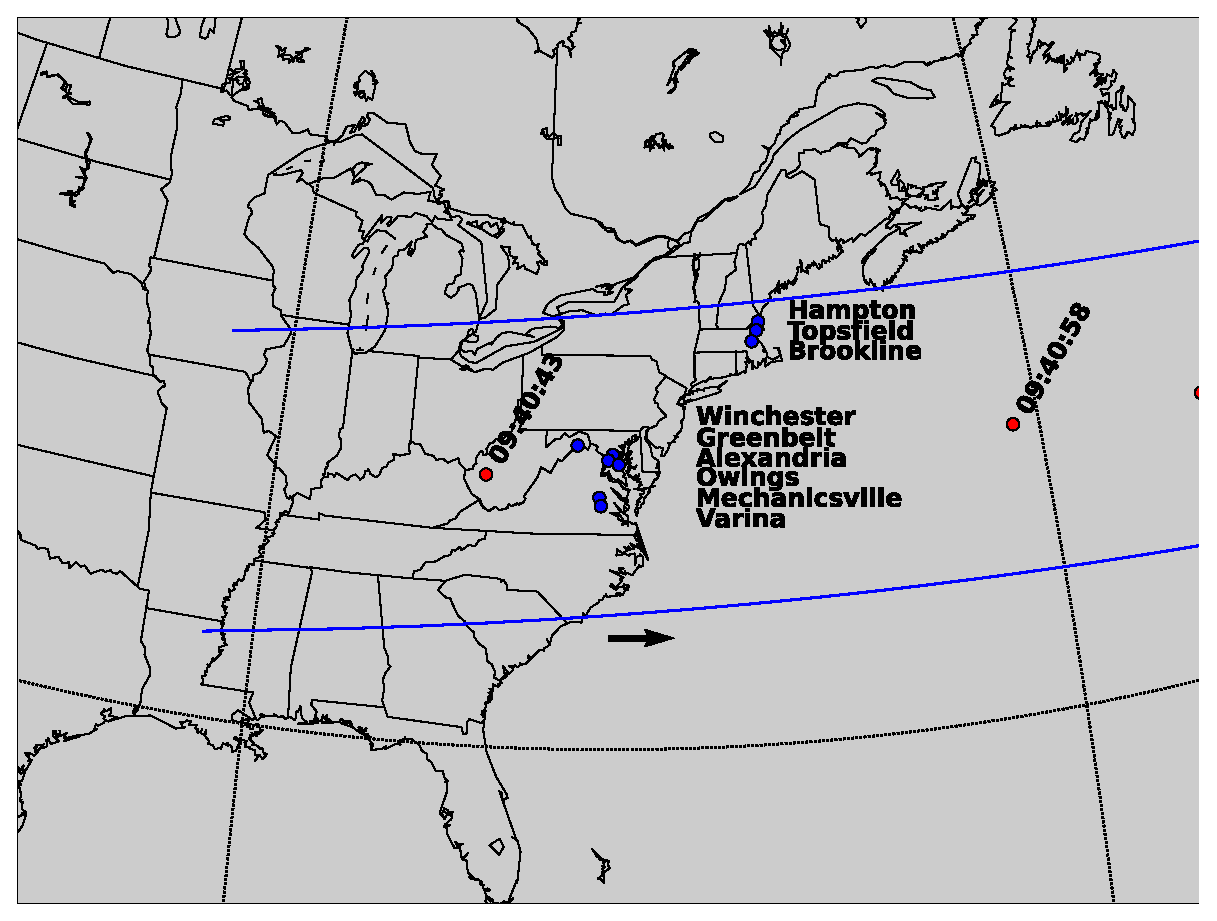
\includegraphics[scale=0.39]{figuras/Ceres_2013-zoom.eps}\label{Fig: Ceres-map-2013}}
\caption{Reconstrução pós-ocultação do caminho da sombra de Ceres na Terra para os eventos de 17 de Agosto de 2010 (a) e 25 de Outubro de 2013 (b). Os pontos em azul são os sítios que observaram os eventos. a) O ponto grande vermelho é a máxima aproximação geocêntrica às 22:40:25 UT. Os pequenos representam o centro da sombra separados por um minuto. b) Visão superior da ocultação sobre os sítios que observaram o evento de 25 de Outubro de 2013. Os pontos vermelhos são os centros da sombra separados por 15 segundos. Nos dois eventos a sombra se move da esquerda para a direita.
\label{Fig: Ceres-map}}
\end{centering}
\end{figure}

\subsection{Ocultação de 2010}
\label{Subsec: 2010-occ}

\indent \indent Em 17 de Agosto de 2010 Ceres ocultou a estrela TYC 6833-163-1 (UCAC4 313-111823), cuja magnitude é $V = 11.55$ e tem posição no ICRS para a data do evento baseada no catálogo UCAC4 \citep{Zacharias2013}:

\begin{equation}
\left\{ 
  \begin{array}{l l}
    \alpha = 17^{h}18^{m}29\fs 0085\\
    \delta = -27\degr 26\arcmin 38\farcs 867
  \end{array}
\right.
\label{Eq: 2010-coord}
\end{equation}

\indent O evento foi observado no Brasil a partir de cinco diferentes sítios (ver Fig. \ref{Fig: Ceres-map-2010}). Destes, 4 obtiveram cordas positivas enquanto UFSC teve uma corda negativa. Das positivas, a observação proveniente do INPE iniciciou-se após o início do evento devido a dificuldades técnicas e, portanto, apenas a emersão da curva de luz foi detectada.

Uma das características mais importantes desse evento foi a velocidade com que ocorreu (apenas 3.9 km s$^{-1}$) acarretando que mesmo exposições de poucos segundos representariam resoluções espaciais significantes.

Todas as observações foram feitas com a utilização de CCDs. As curvas de luz de cada observação foram obtidas das imagens FITS com a utilização do pacote PRAIA \citep[Plataforma de Redução Astrométrica de Imagens Astronômicas,][]{Assafin2011}. As curvas foram normalizadas para o fluxo da estrela mais Ceres, uma vez que eles estavam indistinguíveis logo antes e depois da ocultação. Por fim, elas foram normalizadas pelo ajuste de uma curva polinomial (de primeira ou segunda ordem) fora da queda de fluxo assim fixando em 1 a razão de fluxo fora da ocultação.

Os instantes de ingresso e egresso foram obtidas de cada curva de luz ajustando-se um modelo de poço quadrado levando em consideração a difração de Fresnel, a banda do CCD, o diâmetro aparente da estrela e o tempo de exposição utilizado \citep[ver][]{Widemann2009, Braga-Ribas2013}.

O menor tempo de integração usado nas observações positivas foi de $1.0s$, que corresponde a aproximadamente $3.9km$ no plano do céu. Portanto, o erro na determinação dos instantes de ingresso e egresso é dominado principalmente pelo tempo de integração, não pela difração de Fresnel ou diâmetro da estrela, ambos da ordem de algumas centenas de metros para esse evento.

O ajuste dos dados da ocultação consiste em minimizar uma função dep $\chi^{2}$ clássica para cada curva de luz, como descrito em \cite{Sicardy2011} e \cite{Braga-Ribas2013}. Os parâmetros livres para ajustar são os instantes de ingresso e egresso que fornece o valor mínimo de $\chi^{2}$ ($\chi^{2}_{min}$). O melhor ajuste das curvas de luz para a ocultação de 2010 está mostrado na Fig. \ref{Fig: Ceres-2010-curves}.

\begin{figure}[h]
\begin{centering}
\subfigure[Ocultação de 2010]{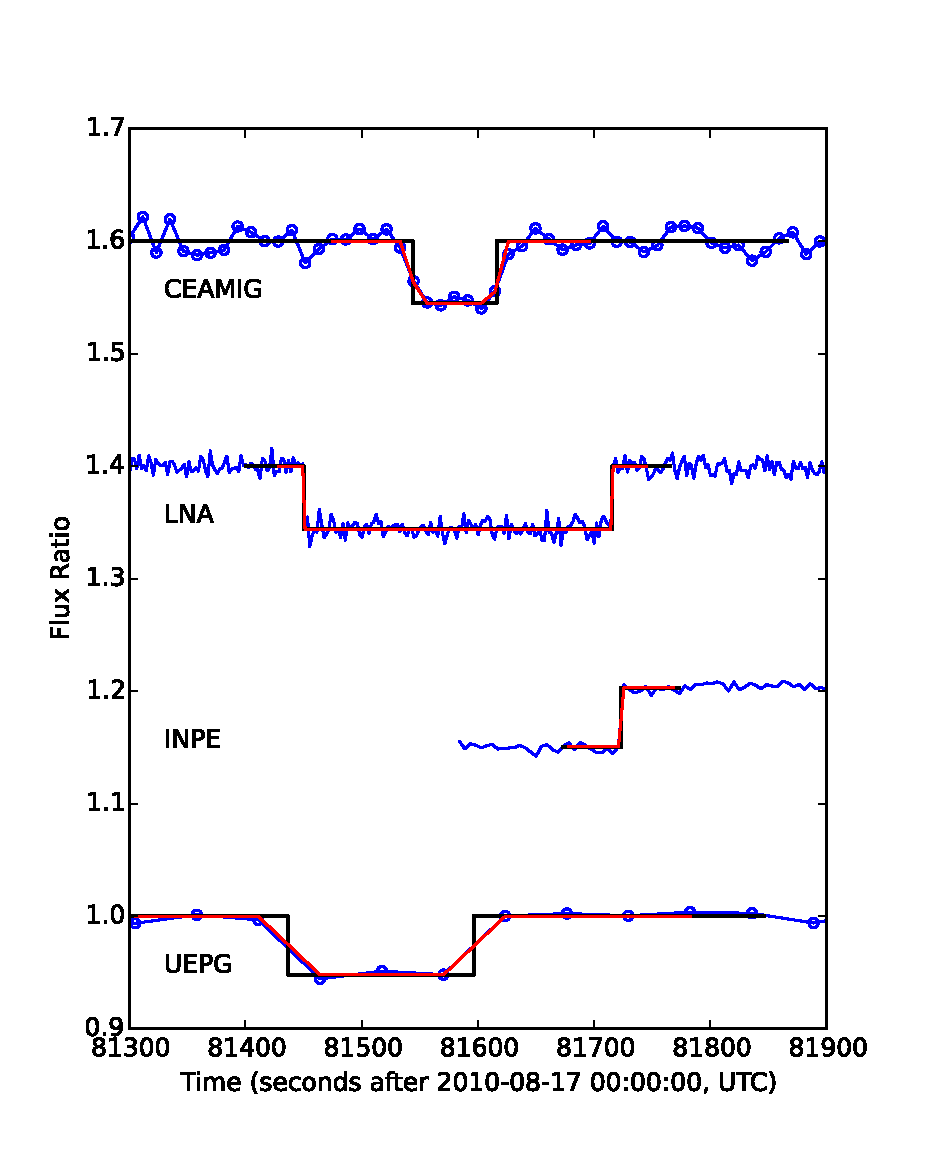
\includegraphics[scale=0.51]{figuras/Ceres_2010_fluxratio.eps}\label{Fig: Ceres-2010-curves} }
\subfigure[Ocultação de 2013]{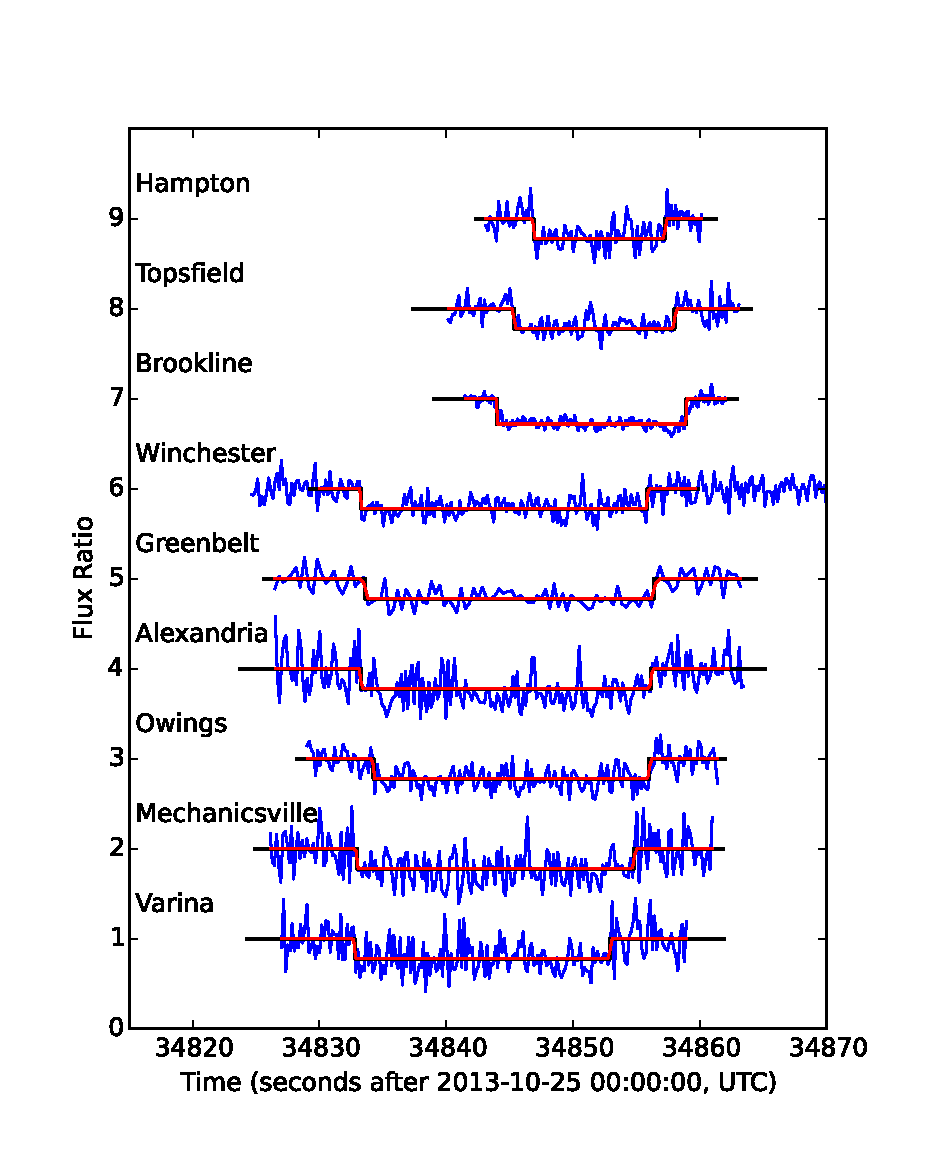
\includegraphics[scale=0.51]{figuras/Ceres_2013_fluxratio.eps}\label{Fig: Ceres-2013-curves} }
\caption{Curvas de luz normalizadas das cordas positivas dos eventos. As curvas estão desviadas por um fator de 0.2 (a) e 1.0 (b) para melhor visualização. As linhas pretas são os melhores ajustes com o modelo de poço quadrado. As linhas vermelhas são os melhores ajustes com o modelo de poço quadrado, porém levando em conta a difração de Fresnel, o diâmetro da estrela e o tempo de exposição. Os instantes médios de cada curva não coincidem devido às diferentes longitudes dos sítios. A curva de luz de Brookline (b) está desviada por um fator de -64 s como explicado no texto.
\label{Fig: Ceres-curves}}
\end{centering}
\end{figure}

A metodologia usada para analizar o perfil de Ceres a partir das observações é o mesmo descrito em \cite{Sicardy2011} e \cite{Braga-Ribas2013}. Cada combinação de posição do sítio, instantes de ingresso e egresso, junto com as coordenadas da estrela e as efemérides de Ceres, correspondem a um ponto no plano do céu. A coleção de todos esses pontos determina o limbo aparente de Ceres.

Adotamos um modelo elíptico para o perfil do limbo, resultante da projeção de um esferóide com achatamento nos pólos no plano do céu. Essa escolha é suportada pelo trabalho de \cite{Drummond2014}, por meio de imagem direta de Ceres. Dessa forma, nós temos $N=7$ extremidades das cordas para ajustar $M=5$ parâmetros que definem uma elipse: semi-eixo maior e semi-eixo menor aparentes ($a^\prime$ and $b^\prime$, respectivamente), ângulo de posição $P$ do seu semi-eixo maior e as posição $(f_c,g_c)$ do seu centro com respeito à estrela ocultada. O semi-eixo maior {$a^\prime$} é equivalente ao raio equatorial $R_{equa}$ do elipsoide.

As coordenadas $f_{c}$ e $g_{c}$, em quilômetros, foram calculadas usando a efeméride de Ceres JPL\#33 \citep{Giorgini1996} e a posição da estrela ocultada. Elas são positivas na direção Leste e Norte celestes, respectivamente. O ângulo de posição $P$ é contado positivamente a partir do norte celeste local em direção ao leste celeste. O achatamento aparente pode ser definido por $\epsilon^\prime = 1 - (b^\prime/a^\prime)$. O melhor ajuste é obtido minimizando uma função de $\chi^{2}_{r}$ reduzido, onde definimos o número de graus de liberdade do problema como $\mathcal{N} \equiv N - M$. Todos os procedimentos que permitem a determinação das barras de erro dos paramêtros físicos podem ser encontradas em \cite{Braga-Ribas2013}.

Duas possíveis soluções foram consideradas para o ajuste do limbo. O primeiro, que chamamos de solução nominal, consiste em determinar os cinco parâmetros que caracterizam uma elipse a partir dos sete contatos observados. A segunda solução consiste em calcular o ângulo de posição $P$ a partir das coordenadas do pólo de Ceres obtidas por \cite{Drummond2014} ($\alpha_{p} = (287 \pm 3) \degr$, $\delta_{p} = (+64 \pm 3) \degr$ no ICRS) e da efeméride de Ceres no instante da ocultação. Chamamos de solução de pólo fixo.

Para o evento de 2010, a solução nominal teve como melhor ajuste $\chi^2_{r,min} = 0.24$, que podem ser interpretadas como as barras de erro estarem superestimadas com respeito à boa qualidade do ajuste. Porém, como o problema tem somente dois graus de liberdade, $\chi^2_{r,min}$ relativamente pequenos são aceitáveis. Os resultados obtidos para o diâmetro equatorial, achatamento, ângulo de posição e coordenadas do centro esao apresentadas na segunda coluna da tabela \ref{Tab: resultados}.

\begin{table}[h]
 \begin{centering}
  \caption{Resultados do ajuste de limbo de Ceres com os dados dos eventos de 2010 e 2013.\label{Tab: resultados}}
  \begin{tabular}{@{}lcccc}
  \hline
     Solution & 2010/Nominal & \textbf{2010/Pólo fixo} & 2013/Nominal & 2013/Pólo fixo \\
\hline
Diam. equat.  (km) & 982 $\pm$ 14 & \textbf{972 $\pm$ 6}  & 971 $\pm$ 7  & 971 $\pm$ 7\\
%Equatorial radius (km) & 491 $\pm$ 7  & \textbf{486 $\pm$ 3}  & 485.5 $\pm$ 3.5 & 485.5 $\pm$ 3.5\\
Achatamento        & 0.08 $\pm$ 0.03 & \textbf{0.08 $\pm$ 0.03} & 0.08 $\pm$ 0.04 & 0.08 $\pm$ 0.04\\
Âng. de pos. (deg)   & 5 $\pm$ 10    & \textbf{12 $\pm$ 3} (*)& 22 $\pm$ 5    & 25 $\pm$ 3 (*)\\
$f_c$ (km)             & 97 $\pm$ 9   & \textbf{102 $\pm$ 5}   & 77 $\pm$ 6    & 78 $\pm$ 6\\
$g_c$ (km)             & 16 $\pm$ 15  & \textbf{21 $\pm$ 11}  & 13 $\pm$ 16   & 13 $\pm$ 16\\
$\chi^2_{r,min}$       & 0.24          &  \textbf{0.42}         & 1.27          & 1.27\\
\hline
\end{tabular}
\textbf{Notas:} Em negrito destaca-se a melhor solução obtida. As barras de erro estão no nível de 1$\sigma$. O diâmetro polar ($D_{pol}$) pode ser facilmente calculado a partir de $D_{pol}=D_{equa}(1 - \epsilon)$. (*) Ângulos de posição derivados a partir das coordenadas do pólo de Ceres determinapas por \cite{Drummond2014}.
\end{centering}
\end{table}

Como pode ser visto, o parâmetro com a maior incerteza é o ângulo de posição cobrindo um intervalo de 20$\degr$. Claramente, fixar as coordenadas do pólo pode melhorar a solução. Por fim, a correção do achatamento devido ao ângulo do aspecto polar está dentro da barra de erro 1$\sigma$ e não tem relevância estatística, dessa forma $\epsilon = 0.08 \pm 0.03$.

No momento da ocultação, as coordenadas do pólo de Ceres correspondiam a um ângulo de posição $P = (12 \pm 3)\degr$. Explorar o espaço de parâmetros restringindo a elipses com ângulo de posição dentro deste intervalo resulta na solução de pólo fixo. O parâmetros físicos do melhor ajuste estão mostrados na Tab. \ref{Tab: resultados} enquanto a solução está esquematizada na Fig. \ref{Fig: Ceres-limb-2010}.

Essa solução corresponde ao limite superior da barra de erro 1$\sigma$ da solução nominal para $P$. Por outro lado, ela obtem os menores valores para o diâmetro equatorial, melhorando sua determinação por um fator de 2.

\begin{figure}[h]
\begin{centering}
\subfigure[Ocultação de 2010]{\includegraphics[scale=0.35]{figuras/Ceres_2010_sphere.eps}\label{Fig: Ceres-limb-2010} }
\subfigure[Ocultação de 2013]{\includegraphics[scale=0.35]{figuras/Ceres_2013_sphere.pdf}\label{Fig: Ceres-limb-2013} }
\caption{Melhores ajustes elípticos para as cordas das ocultações de 2010 e 2013. As setas indicam a direção de movimento, as linhas azuis são as cordas observadas, os segmentos vermelhos são as barras de erro dos ingressos, egressos e centro da ocultação em $1\sigma$. A linha verde em (a) é uma corda negativa. Os instantes marcados em verde em (b) não foram utilizados para o ajuste, como descrito no texto.
\label{Fig: Ceres-limb}}
\end{centering}
\end{figure}


\subsection{Ocultação de 2013}
\label{Subsec: 2013-occ}

\indent \indent Em 25 de Outubro de 2010, Ceres ocultou a estrela TYC 865-911-1 (UCAC4 496-058191), de magnitude $V = 10.05$. Baseada no UCAC4 \citep{Zacharias2013}, sua posição ICRS para a data da ocultação é:

%
\begin{equation}
\left\{ 
  \begin{array}{l l}
    \alpha = 11^{h}57^{m}52\fs7641\\
    \delta = +09\degr 07\arcmin 49\farcs835
  \end{array}
\right.
\end{equation}
%
Esse evento foi observado na costa Leste dos Estados Unidos logo antes do amanhecer, como mostrado na Fig. \ref{Fig: Ceres-map-2013}.

Nove cordas positivas foram obtidas em vários sítios (ver Fig. \ref{Fig: Ceres-map-2013}). Cada estação foi equipada com uma câmera de vídeo com tempo de leitura desprezível. Isso é particularmente importante, já que a velocidade da sombra de Ceres para esse evento foi de 42.6 km s$^{-1}$, muito mais rápido que o evento de 2010.

Durante o evento Ceres estava muito baixo no céu com alturas entre $15\degr$ (Winchester) e $20\degr$ (Hampton). Forte cintilação era esperada e, combinada com o curto tempo de integração e baixa diminuição de brilho, resultou em curvas de luz ruidosas e assim grandes incertezas nos instantes de imersão e emersão.

Todos os vídeos foram convertidos para imagens FITS e a fotometria foi obtidia via \textsc{praia} \cite{Assafin2011}. As curvas de luz foram normalizadas por uma estrela de referência quando havia uma estrela no campo.

Para reduzir o ruído, os dados foram binados por grupos de cinco imagens -- com exceção de Greenbelt, onde gupos de dez imagens foram utilizadas. Esse procedimento o tempo de integração efetivo por um fator de 5 (ou 10). Da mesma forma que para o evento de 2010, uma normalização adicional por um polinômio foi aplicada.

Os instantes de ingresso e egresso da ocultação foram obtidos pelo mesmo procedimento descrito na seção \ref{Subsec: 2010-occ}. Uma vez que o tempo de integração efetivo usado (0.17 s) representa aproximadamente 7 km no plano do céu, e a escala de Fresnel e  o diâmetro da estrela estão novamente na ordem de centenas de metros, o erro da determinação dos instantes de imersão e emersão são dominados principalmente pelo tempo de integração, da mesma forma que para o evento de 2010. Os melhores ajustes para as curvas de luz da ocultação estão mostrados na Fig. \ref{Fig: Ceres-2013-curves}.

Uma comparação entre os tempos obtidos pela estação de Brookline e o restante mostrou que esses têm um atraso de aproximadamente 64 s. Dessa forma, não utilizamos os tempos de Brookline na análise.

Perfis elípticos foram ajustados para todas as cordas restantes. pelo mesmo procedimento descrito na seção \ref{Subsec: 2010-occ}. O resultado foi $\chi^2_{r,min} = 13$ , sugerindo que um modelo elíptico não é satisfatório para os dados. De fato, ao olharmos para a Fig. \ref{Fig: Ceres-limb-2013} vemos que a corda de Varina adiantada com respeito às outras. Como nessa estação o tempo não foi inserido diretamente nos frames do vídeo é possível que essa diferença seja oriunda de um eventual problema da correspondência entre os tempos do camcorder e do GPS.

A imersão gravada em Owings também parece atrasada com respeito às cordas próximas (ver Fig. \ref{Fig: Ceres-limb-2013}). Essa corda tem aproximadamente o mesmo tamanho da corda de Mechanicsville, apesar de estarem separadas por cerca de 100 km. Diferentemente de Varina, essa estação teve os tempos inseridos em cada frame do vídeo o que torna mais difícil justificar um problema de tempo. Outras possibilidades seriam uma má determinação dos instantes de ingresso e egresso dessa curva ou uma característica do relevo de Ceres.

Em um segundo ajuste, não consideramos as cordas de Brookline, Varina e Owings. O ajuste dos cinco parâmetros que definem uma elipse para os doze contatos resultou em $\chi^2_{r,min} = 1.27$, indicando  que está em bom acordo com os dados observados dentro das barras de erro. Essa é a solução mostrada na Fig. \ref{Fig: Ceres-limb-2013}, onde podemos ver que o tamanho da corda de Brookline é compatível com o modelo.

Os resultados das soluções nominais e de pólo fixo não são significantemente diferentes. Isso se deve ao fato da barra de erro do ângulo de posição da solução nominal (que é muito menor que o da solução nominal de 2010) ser muito similar à barra de erro do ângulo de posição da solução de pólo fixo ($P = (25 \pm 3)\degr$). Os dois resultados estão apresentados nas colunas 4 e 5 da tabela \ref{Tab: resultados}.

Sobre a hipótese do atraso observado na imersão da curva de luz de Owings ser associado a uma característica topográfica, o contato gravado corresponderia a uma elevação negativa de 31 $\pm$ 4 km com respeito à elipse de melhor ajuste. Porém modelos teóricos prevêem que relevos em Ceres não devem ser maiores que 10--20 km \citep{Johnson1973}, enquanto dados observacionais limitam o contorno em 18 km \citep{Carry2008}. Imagens mais recentes da sonda \textit{Dawn} também revelam uma superfície mais suave. Portanto, a associação da imersão em Owings com um relevo é improvável.

\subsection{Discussão}

\indent \indent Os resultados apresentados na tabela \ref{Tab: resultados} mostram um acordo entre os parâmetros físicos obtidos nas duas ocultações, especialmente no diâmetro equatorial. As diferenças ocorrem basicamente nos tamanhos das barras de erro e podem ser justificadas pelas particularidades de cada conjunto de dados.

O evento de 2010, por exemplo, teve somente sete contatos, porém bem distribuídos sobre o disco de Ceres. Por outro lado, o evento de 2013 teve cinco contatos a mais, todavia concentrados em certas regiões do corpo. Em particular, a ausência de cordas prómimas ao pólo sul fez seu achatamente ser pior determinado para o evento de 2013 que para o evento de 2010. Mesmo nossa melhor medida de achatamento, $\epsilon=0.08 \pm 0.03$, tem alta incerteza se comparado com outros valores publicados na literatura, como mostra a tabela \ref{Tab: Ceres-final}.

Como foi mostrado, usar as coordenadas do pólo de Ceres determinadas por \cite{Drummond2014} para limitar o ângulo de posição não foi um procedimento eficiente para o evento de 2013. Por outro lado, fixar o ângulo de posição para a ocultação de 2010 reduziu as barras de erro dos outros parâmetros (com exceção do achatamento). Por fim, Esse procedimento resultou em um excelente acordo entre os raios equatoriais obtidos para ambos os eventos.

Uma comparação do diâmetro equatorial de Ceres medido por diferentes técnicas está mostrado na tabela \ref{Tab: Ceres-final}. Vemos um acordo entre os nossos resultados e aqueles obtidos por imageamente direto do Hubble Space Telescope (HST) \citep{Thomas2005}, do Keck Observatory e do ESO VLT \citep{Drummond2014}. O menor valor, reportado por \cite{Carry2008}, pode ser justificado pelo fato desse estudo não levar em conta o efeito de escurecimento de bordo.

O evento de 1984 \citep{Millis1987} é a única outra ocultação que podemos comparar nosssos resultados. As medidas do diâmetro não se acordam dentro de 2$\sigma$. É difícil dizer com certeza as razões dessa divergência. Uma forma de clarificar o problema seria redeterminar os instantes de imersão e emersão das curvas de luz originais usando a mesma metodologia aplicada nesse trabalho. Infelizmente, não temos acesso aos dados da curva de luz original do evento de 1984.

A sonda da NASA \textit{Dawn} poderá responder esses questões que são importantes não só no conhecimento do próprio Ceres, mas também para calibrar todas as técnicas usadas até agora para o estudo das propriedades físicas dos pequenos objetos do Sistema Solar, como as ocultações estelares.

\begin{table}[h]
  \caption{Diâmetro equatorial e achatamento de Ceres \label{Tab: Ceres-final}}
  \begin{centering}
  \begin{tabular}{@{}lccc}
  \hline
     Diâmetro Equatorial (km) & Achatamento & Método & Ref. \\
\hline
$972 \pm 6$  & $0.08  \pm 0.03$  & Occultação & 1\\
$967 \pm 10$ & $0.078 \pm 0.015$ & Keck+VTL    & 2\\
$959 \pm 5$  & $0.074 \pm 0.007$ & Keck        & 3\\
$975 \pm 4$  & $0.067 \pm 0.005$ & HST         & 4\\
$959 \pm 5$  & $0.05  \pm 0.01$  & Occultação & 5\\
\hline
\end{tabular}
\par\end{centering}
\textbf{Referências.} 1: \cite{GomesJunior2015-Ceres}. 2: \cite{Drummond2014}. 3: \cite{Carry2008}. 4: \cite{Thomas2005}. 5: \cite{Millis1987}.
\end{table}


\section{Satélites Irregulares}
\label{Sec: Irregulares}

\subsection{Predição das ocultações}
\label{Subsec: Irr-predic}

\indent \indent Com o objetivo de obter parâmetros físicos para os satélites irregulares com maior precisão foram feitas predições de ocultações estelares para os 7 maiores satélites de Júpiter, o satélite Phoebe de Saturno e Nereida de Netuno. Esses objetos são pequenos (ver Tabela \ref{Tab: comparison-horizons}), se comparados aos TNOs e Centauros estudados na seção \ref{Sec: TNO-occ}, sendo que o menor dos satélites da amostra, Ananke, possui aproximadamente 28 km.

As predições foram feitas utilizando o catálogo UCAC4 e efemérides do JPL. Um total de 588 eventos foram obtidos entre 01 de Janeiro de 2015 e 31 de Dezembro de 2017 para os 9 objetos sendo que a maioria será descartada por passar em regiões de oceano ou onde não há observadores disponíveis. Para Nereida, apenas uma estrela UCAC4 foi identificada para ser ocultada. Nesse caso, utilizamos um catálogo de estrelas feito a partir do caminho aparente do satélite de Netuno Tritão no céu para predições de ocultações estelares pelo mesmo (ver seção \ref{Sec: TNO-occ}).

Como esses objetos são muito pequenos, em sua maioria as ocultações durarão poucos segundos, portanto apenas eventos com estrelas brilhantes serão selecionados e se houver câmeras de integração rápida disponíveis. Por outro lado, os satélites de Júpiter estão muito mais pertos que os TNOs e como o erro astrométrico é uma medida angular, consequentemente, o erro da sombra da ocultação projetada na Terra será muito menor que aquelas medidas para TNOs. Assim, a área a ser coberta para que uma ocultação por satélite irregular de Júpiter seja detectada será da ordem de poucas centenas de quilômetros.

\subsection{Testes}
\label{Subsec: Irr-testes}

\indent \indent Até que o primeiro catálogo GAIA seja lançado, as posições das estrelas usadas serão as do catálogo UCAC4. Porém esse catálogo possui imprecisões relevantes principalmente para as estrelas mais fracas. Uma das estrelas testadas apresentou um offset da posição do catálogo para a data da observação de mais de 600 mas. Para a estrela em questão, esse valor representa uma variação de aproximadamente 1900 km da sombra projetada na Terra.

Para corrigir esses erros, será necessário observar as estrelas a serem ocultadas dias antes do evento obtendo os offsets correspondentes e calibrando a predição. Erros em ascensão reta interferem majoritariamente no instante em que a ocultação ocorrerá. Já erros em declinação principalmente na latitude geográfica em que a sombra passará.

Outra fonte de erro na predição é a posição do satélite. Como mostradas no capítulo \ref{Cap: Irr-astrometria}, as órbitas dos satélites irregulares não são muito precisas havendo erros sistemáticos em seus elementos orbitais. Infelizmente o JPL não provê suas efemérides com os erros estimados das posições. Dessa forma, há três alternativas para a correção das posições dos satélites.

A primeira delas é observar o satélite dias antes, quanto mais próximo do evento melhor, e determinar um offset. O offset, portanto, seria considerado estável dentro desses poucos dias uma vez que ele não se move muito em sua órbita. Porém, nem sempre é possível observar o alvo com antecedêndia.

A segunda alternativa é recalcular as órbitas dos satélites, gerar novas efemérides e estimar seus erros. Espera-se que com o grande número de posições publicadas em \cite{GomesJunior2015-Irregular} as órbitas sejam calculadas com maior precisão. Esse integração numérica será trabalhada durante o doutorado sanduíche em Paris em colaboração com o Dr. Jean-Eudes Arlot e o Dr. Josselin Desmars. Um trabalho semelhante foi abordado para ocultação de Centauros e TNOs (ver seção \ref{Sec: TNO-occ}).

Por fim, a terceira alternativa consiste em se fazer um ajuste dos offset obtidos em \cite{GomesJunior2015-Irregular} em função da anomalia verdadeira, tempo e/ou anomalia média. Essa escolha é suportada pelas dispersões dos offsets em função da anomalia verdadeira (por exemplo, Fig. \ref{Fig: carme_anom}, para Carme) que apresentaram características notáveis. Os parâmetros a serem utilizados para cada satélite serão estudados e aplicados. Esse é o método que será utilizado para o artigo de predições de satélites irregulares que será submetido logo.

Os primeiros ajustes foram feitos apenas considerando os offsets em declinação, pois são os que apresentaram características mais evidentes e, por seus erros representarem principalmente erros em latitudes, são os principais responsáveis pela não detecção da ocultação. Nesse caso, utilizamos um ajuste em função de três parâmetros: sen${f}, \cos{f}$ e uma constante, onde $f$ é a anomalia verdadeira dada pela efeméride. Esse ajuste é mostrado na Fig. \ref{Fig: Carme-dec-fit}.

\begin{figure}
\begin{centering}
\includegraphics[scale=0.45]{figuras/Carme-DEC_fit.png} 
\caption{Ajuste dos offsets em declinação de Carme publicados em \cite{GomesJunior2015-Irregular} em função da anomalia verdadeira}
\label{Fig: Carme-dec-fit}
\end{centering}
\end{figure}

É possível ver para o caso de Carme que o ajuste representa razoavelmente bem a dispersão dos offsets em função da anomalia verdadeira. Para outros satélites, ajuste em primeira ordem do seno e do cosseno da anomalia verdadeira também representam razoavelmente bem os offsets em declinação. Para os offsets em ascenção reta, o ajuste com três parâmetros não é suficiente.

Observar uma ocultação estelar de um satélite irregular exige um esforço muito grande por parte dos observadores. A sombra cobrirá uma região muito restrita na Terra devido aos satélites irregulares serem pequenos. Portanto, antes de iniciar uma grande campanha observacional, testaremos algumas ocultações, principalmente dos objetos maiores para confirmar a predição.

Esse teste consiste em se observar o objeto ocultante e a estrela a ser ocultada próximo ao evento, quando os dois objetos estiverem presentes no mesmo campo, preferencialmente próximo ao instante do evento quando os objetos estarão o mais próximo possível. Assim as posições relativas entre os dois objetos terá mínima influência dos erros das estrelas de catálogo utilizadas na redução e das possíveis distorções de campo.

Até o momento, apenas dois testes de ocultações foram feitas, uma de Himalia que ocorreu dia 03 de Março de 2015 e a segunda de Elara que ocorreu dia 30 de Março de 2015. Para cada evento quatro mapas foram gerados: o primeiro com as posições nominais da estrela e do satélite para o instante previsto; a segunda com o offset calculado como descrito anteriomente; o terceiro com os offsets da estrela e do satélite a partir de observações feitas alguns dias antes da ocultação quando os dois objetos estavam separados (campos diferentes); e o quarto a partir de observações feitas com menos de 24 horas de diferença da data prevista com a estrela e o satélite próximos no mesmo campo.

A Fig. \ref{Fig: occ-Himalia} mostra os quatro mapas para o teste da ocultação de Himalia de 03 de Março de 2015. O mapa \ref{Fig: occ-Himalia-off22fev} foi feito a partir de posições obtidas em 22 de fevereiro observadas no telescópio Zeiss do Observatório do Pico dos Dias (OPD). Nesse dia, Himalia e a estrela a ser ocultada foram observados em campos separados por ainda estarem distantes. Na noite do evento, 03 de março, os objetos foram observados com o telescópio Perkin-Elmer do OPD pouco mais de uma hora após os instante previsto para o evento. Satélite e estrela estavam separados por aproximadamente 16 arcsec, portanto muito próximos no campo. A partir dos offsets calculados, o mapa \ref{Fig: occ-Himalia-off03mar} foi gerado.

\begin{figure}
\begin{centering}
\subfigure[Sem offsets]{\includegraphics[scale=0.16]{figuras/Himalia1_2015-03-03T00:39:25.png}  \label{Fig: occ-Himalia-nooff}}
\subfigure[Offset de Himalia a partir do ajuste]{\includegraphics[scale=0.16]{figuras/Himalia2_2015-03-03T00:39:18.png}  \label{Fig: occ-Himalia-ajuste}}
\subfigure[Obs. dia 22 de Fevereiro (campos separados)]{\includegraphics[scale=0.16]{figuras/Himalia3_2015-03-03T00:39:40.png}   \label{Fig: occ-Himalia-off22fev}}
\subfigure[Obs. dia 03 de Março (mesmo campo)]{\includegraphics[scale=0.16]{figuras/Himalia4_2015-03-03T00:39:15.png}   \label{Fig: occ-Himalia-off03mar}}
\caption{Predições para Himalia. O ponto grande em vermelho mostra o local de máxima aproximação da sombra na Terra, os pontos vermelhos menores são os centros da ocultação separados por um minuto, as linhas retas são os limites das sombras dado o tamanho do objeto e as linhas tracejadas demonstram uma diferença de 40 mas do centro da sombra. (a) é o mapa utilizando apenas as posições nominais da estrela e do satélite. (b) mostra a sombra dado um offset estimado pra posição de Himalia dado sua anomalia verdadeira segundo um ajuste feito em cima dos offsets publicados em \cite{GomesJunior2015-Irregular}. Em (c) são aplicados offsets às posições da estrela e do satélite dado observações feitas em 22 de fevereiro no telescópio Zeiss. Em (d), temos o mesmo que para (c) porém com offsets obtidos de observações feitas em 03 de Março no telescópio Perkin-Elmer quando os objetos estavam próximos no campo}
\label{Fig: occ-Himalia}
\end{centering}
\end{figure}

Para esse evento é possível ver que a sombra não varia muito dentre os quatro mapas sugerindo que para Himalia uma probabilidade maior de observar um evento. De fato, a maior diferença entre as sombras dos quatros mapas é de $25 s$ e $130 km$ na direção perpendicular às sombras.

Na Fig. \ref{Fig: occ-Elara} temos os mapas para a ocultação de Elara do dia 30 de Março. As observações de teste foram tomadas dias 25 de março e 02 de abril no Zeiss. Na noite do dia 02 eles ainda puderam ser observadas no mesmo campo. Devido à Elara ser bem mais fraco, as dispersões das posições do satélite nas duas noites acabaram sendo maiores que para Himalia. Ainda assim, as diferenças entre os mapas obtidos foram pequenos. A maior diferença entre elas é de $48 s$ e $302 km$.

\begin{figure}
\begin{centering}
\subfigure[Sem offsets]{\includegraphics[scale=0.16]{figuras/Elara1_2015-03-30T01:45:15.png} \label{Fig: occ-Elara-nooff}}
\subfigure[Offset de Elara a partir do ajuste]{\includegraphics[scale=0.16]{figuras/Elara2_2015-03-30T01:44:59.png} \label{Fig: occ-Elara-ajuste}}
\subfigure[Obs. dia 25 de Março (campos separados)]{\includegraphics[scale=0.16]{figuras/Elara3_2015-03-30T01:44:17.png}  \label{Fig: occ-Elara-off25mar}}
\subfigure[Obs. dia 02 de Abril (mesmo campo)]{\includegraphics[scale=0.16]{figuras/Elara4_2015-03-30T01:45:30.png}  \label{Fig: occ-Elara-off02abr}}
\caption{Predições para Elara. Mesmo que a Fig. \ref{Fig: occ-Himalia}, mas para Elara. O mapa (c) feito a partir de observações tomadas dia 25 de março e (d) a partir de observações de 02 de abril.}
\label{Fig: occ-Elara}
\end{centering}
\end{figure}

Um pedido de tempo foi feito para o telescópio Zeiss para se tentar observar uma ocultação de Himalia  dia 23 de Outubro de 2015. A sombra dessa ocultação passará pela região sudeste do Brasil (ver Fig. \ref{Fig: occ-Himalia-itajuba}). O evento ocorrerá muito baixo do céu (~22º de altura) e estará próximo ao amanhecer, porém se observar será a primera ocultação de um satélite irregular.

\begin{figure}
\includegraphics[scale=0.35]{figuras/Himalia_2015-10-23T07:54:47.png}
\caption{Mapa da ocultação de Himalia que ocorrerá em 23 de Outubro de 2015}
\label{Fig: occ-Himalia-itajuba}
\end{figure}


\section{Centauros e TNOs}
\label{Sec: TNO-occ}

\indent \indent Como dito no Cap. \ref{Cap: intro}, os objetos do sistema solar exterior podem ser considerados fósseis do sistema solar. Dentre esses, os TNOs, por estarem mais distantes, são os que guardam as informações mais antigas. Ainda é incerta a distribuição de tamanhos dos TNOs e pouco se conhece sobre suas composições, estruturas internas, presença de atmosfera, densidade, etc.

Com o objetivo de obter os parâmetro físicos desses objetos uma grande campanha observacional é realizada para se observar ocultações estelares por TNOs e Centauros (a partir daqui, "TNOs" se referem a TNOs e Centauros). Essa campanha é liderada por pesquisadores brasileiros, franceses e espanhóis e tem colaboração com observadores espalhados por todo o mundo.

Assim como para os satélites irregulares, observar uma ocultação exige um grande trabalho de predição e sua melhoria. Os TNOs estão muito distantes significando que erros pequenos em sua posição ou na posição da estrela podem significar um erro do local onde a sombra irá passar de muitos quilômetros. Preferencialmente, esse erro tem que ser menor que o tamanho angular do objeto no plano do céu. Por exemplo, Plutão tem um raio de $1190 \pm 5$ km \cite[em preparação]{DiasOliveira2015} que a uma distância de aproximadamente 32 UA representam um diâmetro angular de 102 mas. Para a maioria dos objetos selecionados, menores que Plutão e/ou mais distantes, seus tamanhos angulares são manores que 50 mas.

Da mesma forma, estando muito distantes, eles se movem pouco no céu ocultando poucas esrelas, porém sendo menos brilhantes (Mag V > 18) é possível observar ocultações de estrelas mais fracas, onde a queda de brilho da estrela durante a ocultação poderá ser detectada com baixo sinal-ruído.

Para identificar candidatas a ocultações estelares foi realizado uma campanha observacional no ESO para observar os caminhos aparentes dos TNOs entre 2009 e 2015. As observações foram feitas com o telescópio de 2.2 m e o detector mosaico WFI. Posições para estrelas até magnitude R=21, com nível de completeza em R=19, foram obtidas com precisões menores que 20 mas até R=20 \citep{Assafin2012}. Assim, estrelas que não estão no UCAC4, catálogo comumente utilizado como referência astrométrica, foram identificados bem como estrelas que estão mas não tem posições ou movimentos próprios com precisão suficiente. Tantos os catálogos de estrelas quanto as cadidatas a ocultação foram publicados em periódicos \citep{Assafin2010, Assafin2012, Camargo2013}.

Não somente as posições das estrelas precisam ser atualizadas, mas também as posições dos TNOs. Portanto os TNOs também foram observados tanto no ESO quanto No Observatório do Pico dos Dias. À princípio as predições das ocultações eram atualizadas utilizando o método de offsets, porém, em colaboração, integrações numéricas das órbitas dos TNOs foram realizadas desenvolvendo-se uma ferramenta denominada NIMA\footnote{Numerical Integration of the Motion of an Asteroid} \citep[submetido]{Desmars2015}.

Nesse trabalho, posições obtidas de ocultações já realizadas tem um peso muito maior que as restantes, diferentemente do que é feito pelo JPL. Da mesma forma, noites em que houveram um número de observações maior que as restantes terá um peso moderado já que se fosse utilizado um peso individual, o peso final de uma noite poderia estar superestimado levando a um erro na integração. Neste trabalho contribuí com observações de TNOs feitas no OPD.

Vários objetos já foram observados pelo grupo, sendo que o Sistema Plutão-Caronte conta com várias ocultações observadas. Essa trabalho já gerou diversas publicações, incluindo na revista Nature, por exemplo \cite{Sicardy2011} e \cite{BragaRibas2014} nas quais contribuí em caráter observacional. A ocultação de Plutão de 04 de Maio de 2013, a qual observei, gerou duas publicações \citep{Olkin2015, DiasOliveira2015}.

\cite{Sicardy2011} identificaram, a partir de uma ocultação de 06 de Novembro de 2010, que Eris é um planeta anão menor do que se esperava. Devido a seu brilho e distância acreditava-se que ele fosse muito maior, mas na verdade ele tem um albedo geométrico no visível de $p_v=0.96^{+0.09}_{-0.04}$ e que seu tamanho é de $1163 \pm 6$ km, muito próximo ao tamanho de Plutão. O alto albedo de Eris pode ser relacionada à presença de uma atmosfera colapsada devido ao fato dele estar se aproximando de seu afélio.

\cite{BragaRibas2014} observaram uma ocultação do Centauro Chariklo que ocorreu dia 03 de Junho de 2013. O ocultação revelou que o objeto possui um sistema de anéis nunca visto antes em um objeto tão pequeno. Até o momento, conhecia-se apenas anéis em torno dos planetas gigantes. Essa descoberta levanta muitas questão sobre formação dos anéis, estabilididade ou tempo de vida e nos leva a crer que pode haver mais objetos com anéis no sistema solar.

\cite{Olkin2015} determinaram a partir de observações de ocultações por Plutão que a atmosfera do objeto não colapsa durante os 248 anos de sua órbita, como acontece com Eris. Modelos anteriores previam um colapso de sua atmosfera devido a Plutão receber três vezes menos luz do Sol em afélio que em seu periélio.

\cite{DiasOliveira2015}, também a partir de ocultações de Plutão, utilizaram modelos para obter os perfis de temperatura, pressão e densidade da atmosfera do objeto. Os modelos ajustam perfeitamente os perfis de temperatura para as duas ocultações utilizadas assumindo uma atmosfera esfericamente simétrica. Foi obtido que a pressão da atmosfera aumentou cerca de 6\% entre 2012 e 2013 significando que a atmosfera de Plutão ainda está se expandindo e confirmando o trabalho de \cite{Olkin2015}.

No dia 29 de Junho de 2015 haverá uma ocultação de Plutão de máxima importância. Será a última antes da chegada da sonda \textit{New Horizons} no sistema e poderá ser observada na Austrália. Observada a ocultação, os modelos de perfil de atmosfera para Plutão poderão ser calibrados com os dados da \textit{New Horizons} para serem utilizadas em futuras ocultações e estudar a evolução da atmosfera do planeta anão.

Em 29 de Abril de 2014, uma ocultação de Chariklo foi observada na África. Eu trabalhei com a redução de três curvas de luz (Gifberb, SAAO e Springbok). Um fato interessante dessa ocultação foi que a estrela era uma binária não catalogada. Como a segunda estrela era bem mais fraca, acreditava-se que poderia ser algum material próximo à Chariklo.

Essa ocultação foi importante para obter com total certeza a direção do pólo de Chariklo. Além disso, as câmeras utilizadas eram de alta qualidade possibilitando obter que pelo menos um dos anéis é opaco. Uma das cordas, fortuitamente, passou contígua ao anel observando apenas o anel externo. Os resultados ainda não foram publicados.

Outro evento que observei foi uma ocultação de 2003VS2 dia 07 de Novembro de 2014 no OPD. As variações do céu não permitiram uma boa observação de forma que a curva de luz estava muito variada com instantes de tempo bom próximos ao instante do evento. Um trabalho foi feito para identificar alguma ocultação mas nada pôde ser extraído. O trabalho ainda está em análise.



\chapter{Cronograma das Atividades}
\label{Cap: cronograma}

\glsaddall
\printglossary


\bibliography{Referencias}
\bibliographystyle{apalike}


\end{document}
